\documentclass{jarticle}

\usepackage{latexsym}
\usepackage{graphicx}
\usepackage{here}

\title{情報科学演習及び実験1(Java演習)}
\author{IS2 6316047 出納 光}
\begin{document}

\maketitle

\newpage
\section{折れ線グラフ}
\begin{verbatim}
※ データの要素数が多いと横軸に入りきらない恐れがあるため、
10個くらいと一般的な要素数を扱うものとする。

main関数ではウィンドウの描画を行う。
ここでは主に背景色の指定のみを行なっている。

paintComponent関数では、
まず始めにtry内でデータの読み込み行う。
data.txtを引数として中身を読み込み、
readLineで行の読み込み、splitで各行でスペースごとに要素を区切る。
後々使用するため、データの要素の総数xをdata.lengthより求め、
parseIntでString型で読み込まれたデータをint型に変換する。

続いて、折れ線グラフを実装するために、
drawLineとfillRectを用い、横軸及び縦軸、グラフの描画範囲を指定する。
後々使用するため、forループからmaxとminにデータの最大値、最小値を格納する。
次のforループでは要素の数だけ再帰し、横軸のメモリを作る。
続くforループでは再び要素の数だけ再帰し、横軸に要素の順番を表示する。
その次にはforループを5回だけ再帰させ、縦軸を4等分にするメモリを作る。その際に最大値の1/4ずつで指標を示す。
最後のforループではデータの2つの要素の座標をdrawLineで結ぶ。
このとき、「ある要素の値/全データ中の最大値」に縦軸の幅を掛けることでグラフを拡大縮小し、適切なサイズに調整している。

最後にcatchより、ファイルが見つからなかったときのエラーである"NOT_FOUND"、何らかの事情によりファイルが開けなかったエラー"CAN_NOT_OPEN"を返す。

\end{verbatim}

\begin{figure}[H]
\begin{center}
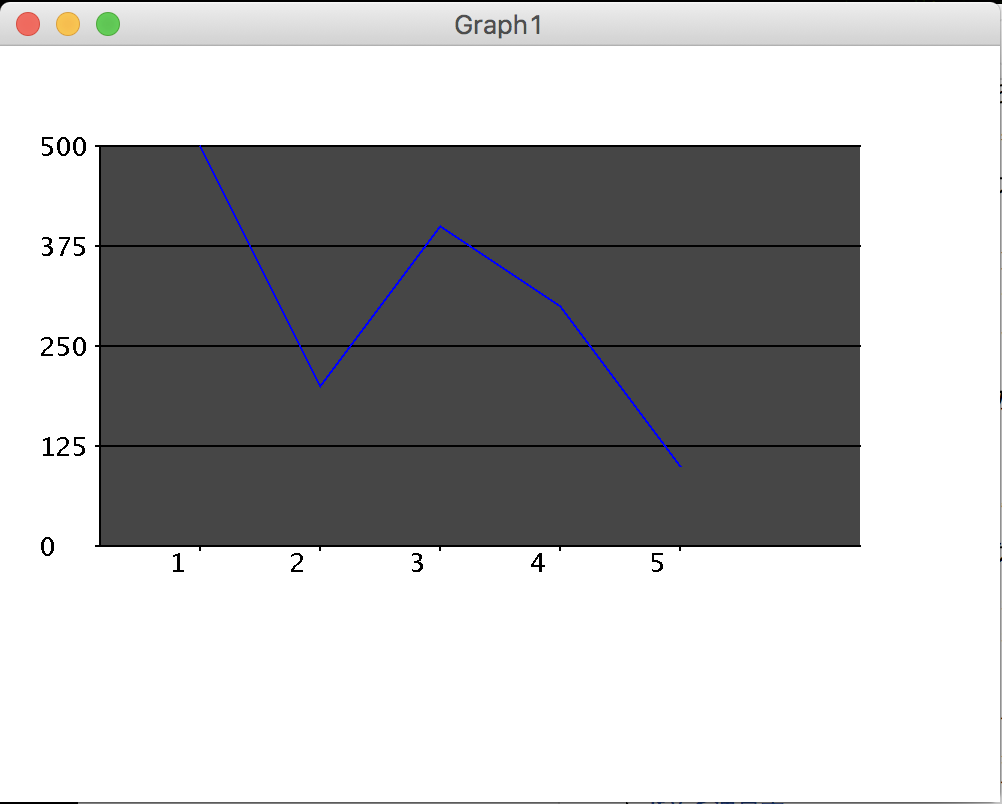
\includegraphics[scale=0.5]{1.eps}
\end{center}
\caption{実行例 1}
\end{figure}

\begin{figure}[H]
\begin{center}
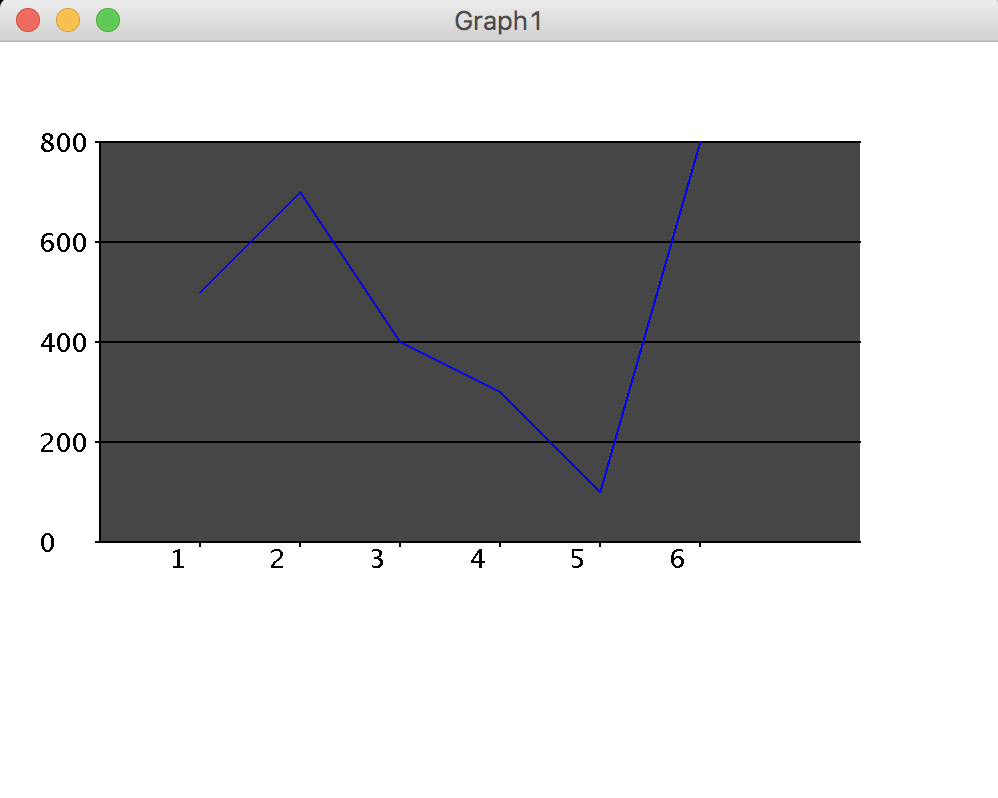
\includegraphics[scale=0.5]{2.eps}
\end{center}
\caption{実行例 2}
\end{figure}

\begin{verbatim}
グラフとして実用的に用いられる品質で描画されている。
それぞれの指標に対して、データの各値は適切な割合を示している。
データの要素数を増やしても、同様に維持される。
データのそれぞれの値の帯域を拡げても、同様に維持される。
\end{verbatim}

\newpage
\section{円グラフ}
\begin{verbatim}
main関数ではウィンドウの描画を行う。
ここでは主に背景色の指定のみを行なっている。

paintComponent関数では、
まず始めにtry内でデータの読み込み行う。
data.txtを引数として中身を読み込み、
readLineで行の読み込み、splitで各行でスペースごとに要素を区切る。
後々使用するため、データの要素の総数xをdata.lengthより求め、
parseIntでString型で読み込まれたデータをint型に変換する。

続いて、円グラフを実装するために、
まず後々用いることとなるため、forループにより全データの合計値sumを求める。
また開始角startを90度に指定し、円グラフが最上部から開始するように設定する。
その後、forループによりデータの要素の数だけ再帰させる。その中で、まずは「ある要素の値/全データの合計値」より、その要素が占める割合rateを示し、
それに360を掛けることでデータの要素1つあたりが占める角度radを求める。
続いて、setColorの引数に0から255までの数値をランダムにRGBとして割り当てる。
fillArcの引数として先ほど用意したstartを開始角として、radを描画角として割り当て、円グラフを描画する。
このとき、円グラフは時計回りであるため、-radとして引数を取ることに注意した。
円グラフの描画の最後に開始角に描画角を足して、次の開始角が続きから始まるようにする。

続くdrawStringでは、データの各値をsin関数とcos関数を用いることで円の周囲に表示する。
さらにどの色がどの要素であるかを示す指標も添付した。
このときには、ランダムで変化する色をsetColorにより黒色で表示することに気をつけた。

最後にcatchより、ファイルが見つからなかったときのエラーである"NOT_FOUND"、何らかの事情によりファイルが開けなかったエラー"CAN_NOT_OPEN"を返す。

\end{verbatim}

\begin{figure}[H]
\begin{center}
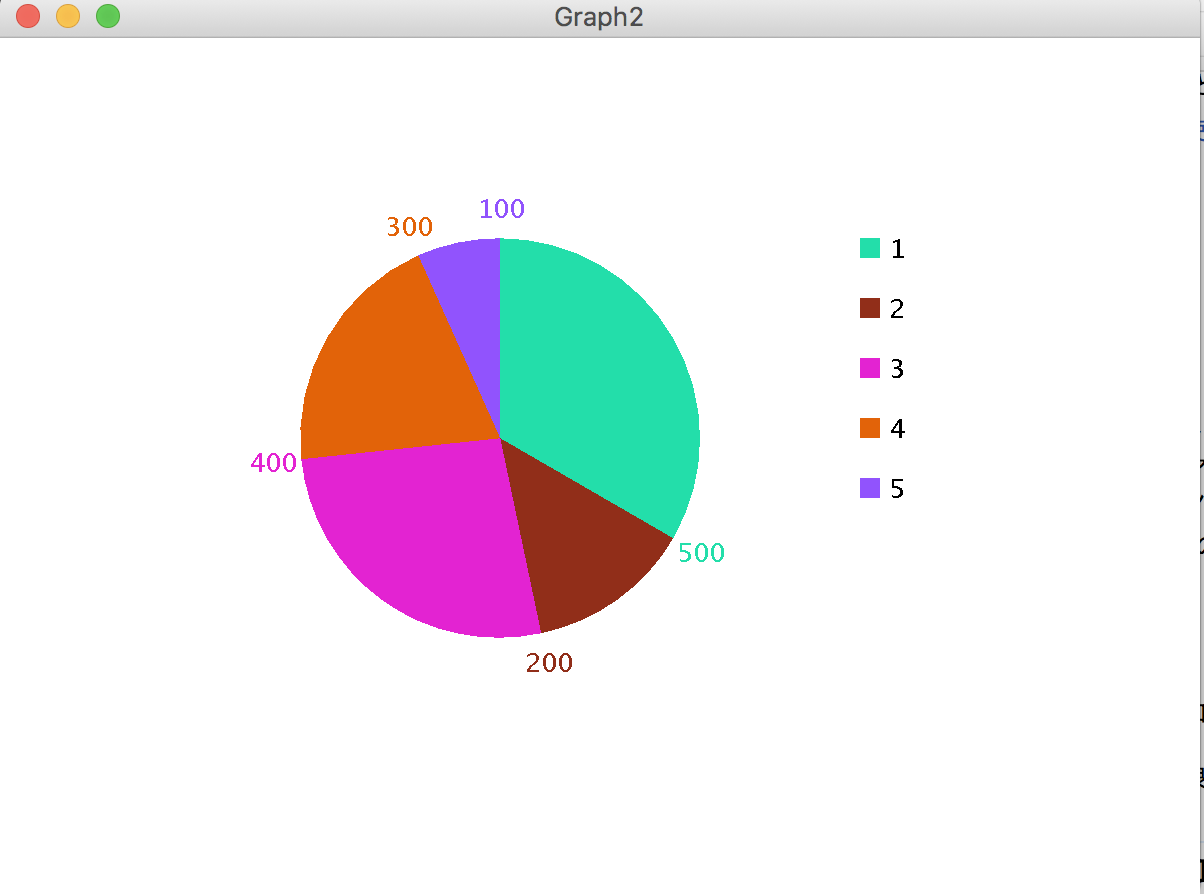
\includegraphics[scale=0.5]{3.eps}
\end{center}
\caption{実行例 1}
\end{figure}

\begin{figure}[H]
\begin{center}
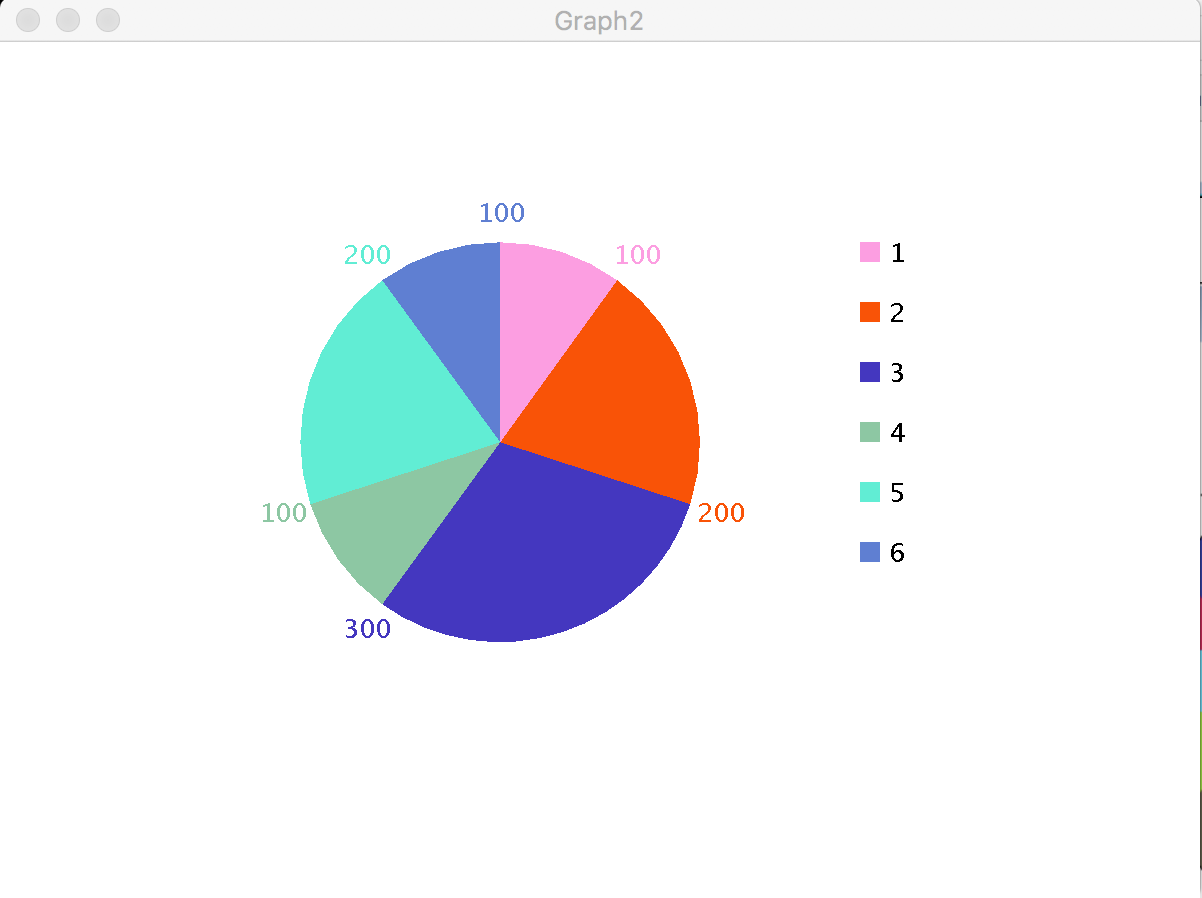
\includegraphics[scale=0.5]{4.eps}
\end{center}
\caption{実行例 2}
\end{figure}

\begin{verbatim}
グラフとして実用的に用いられる品質で描画されている。
それぞれの指標に対して、データの各値は適切な割合を示している。
データの要素数を増やしても、同様に維持される。
データのそれぞれの値の帯域を拡げても、同様に維持される。
\end{verbatim}

\newpage
\section{レーダーチャート}
\begin{verbatim}
main関数ではウィンドウの描画を行う。
ここでは主に背景色の指定のみを行なっている。

paintComponent関数では、
まず始めにtry内でデータの読み込み行う。
data.txtを引数として中身を読み込み、
readLineで行の読み込み、splitで各行でスペースごとに要素を区切る。
catchより、ファイルが見つからなかったときのエラーである"NOT_FOUND"、何らかの事情によりファイルが開けなかったエラー"CAN_NOT_OPEN"を返す。

続いて、レーダーチャートを実装するために、
後々用いるため、まずデータの要素の総数xをdata.lengthより求め、
parseIntでString型で読み込まれたデータをint型に変換する。
forループからmaxとminにデータの最大値、最小値を格納する。
続いてデータの各要素の位置を表示するために、mtxにそのx座標、mtyにそのy座標を配列として割り当てる。
その引数には、「データの各要素の値/全データの最大値」にグラフの描画範囲を幅を掛けることでグラフを拡大縮小し、適切なサイズに調整している。
setColorにより色を変更し、fillPolygonを用いて各要素の占める範囲を描画する。
ここでは、先に範囲を描画し、その後グラフのメモリを描画するという順番で実装しなければ、
実行結果で表示されるグラフの範囲にメモリが上書きされ、見辛くなってしまう点に注意した。

最後に、5段階のメモリに最大値の1/5が指標として表示されるように実装した。
\end{verbatim}

\begin{figure}[H]
\begin{center}
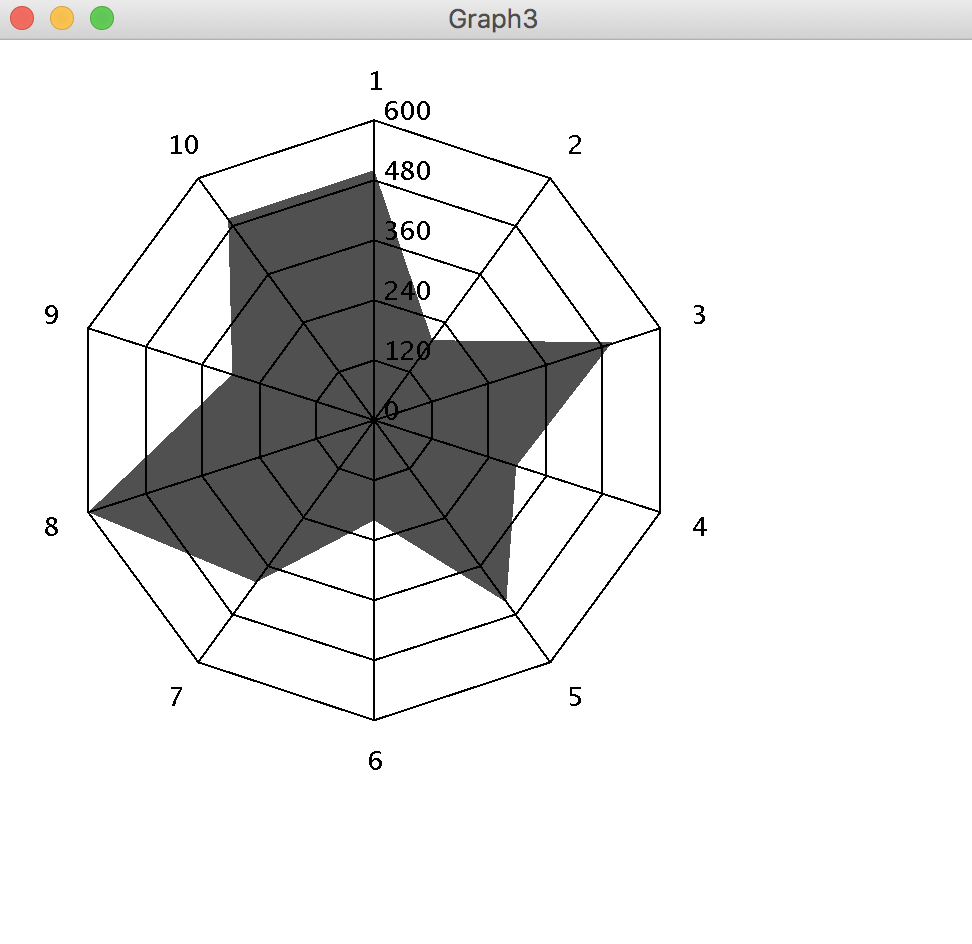
\includegraphics[scale=0.5]{5.eps}
\end{center}
\caption{実行例 1}
\end{figure}

\begin{figure}[H]
\begin{center}
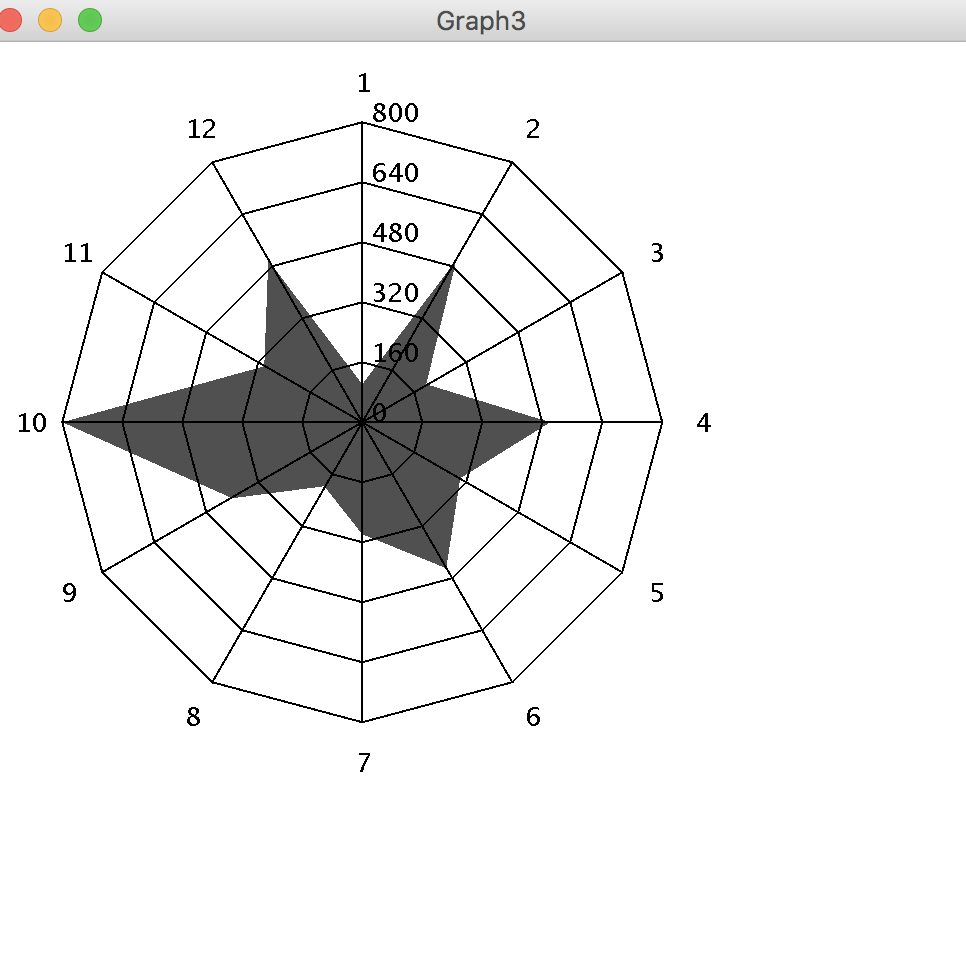
\includegraphics[scale=0.5]{6.eps}
\end{center}
\caption{実行例 2}
\end{figure}

\begin{verbatim}
グラフとして実用的に用いられる品質で描画されている。
それぞれの指標に対して、データの各値は適切な割合を示している。
データの要素数を増やしても、同様に維持される。
データのそれぞれの値の帯域を拡げても、同様に維持される。
\end{verbatim}

\newpage
\section{考察}
\begin{verbatim}
今後のチームで開発していく際の長期的なメンテナンスも見据え、ソースコードに十分な可読性を持たせるためにも、
「分かり易いクラス名及び変数名をつけること」
「コメントアウトを用い補足説明を加えること」
「エラーを状態に応じて細かく分けること」
といったことは勿論、
「コンポーネント単位でまとまりを作ること」や「明示的に変数を宣言すること」が大切である。
\end{verbatim}

\end{document}
